\chapter{List ADT} \label{lists}

\section{Introduction}
       Usually when we write programs we don’t know how many records or data items will be available to the program. Frequently that number isn’t known even when data is entered into the program. Data storage structures like arrays are sometimes inconvenient because the length of an array must be known in order to allocate memory for the structure before data can be entered.     
       
       Linked Data structures solve this problem by allocating exactly enough  memory for a single data item, filling the item, then allocating enough  memory for the next item and connecting the two together so that they form a collection of data items. This process is repeated for however many items there are.     

       These types of constructs are called \textbf{dynamic data structures}. Don’t confuse  this term with dynamic memory allocation- the word dynamic simply means that the action happens as the program is executing.  So dynamic memory allocation (malloc) happens during program execution and a dynamic data structure is created during program execution, but the two things are separate.   
   
   \section{Linked Lists}
       A linked list can be constructed in several different ways.The differences between the construction is in the number and purpose of the pointers in the node structure.  Sometimes all that is needed is a simple list, where the first item in the list leads to the second item which leads to the third item and so on.  This is called a \textbf{singly linked list}.  A singly linked list provides no mechanism to return to the previous item.  Imagine a collaborative story-writing task where each person writes a sentence on paper and then passes the paper to someone else who writes another sentence on the paper.  At the end of the task, there is a story on each piece of paper and the last author is holding the list of sentences, but there is no record of who the previous authors were.  That is how a singly linked list works.
       
       A \textbf{double linked list} provides a mechanism to identify both the next item on the list as well as the previous item on the  list from any position in the list.  A double linked list is similar to a group of people standing in line.  Any individual person can identify both the person ahead of them in the line and the person behind them.
       
       A \textbf{circular linked list}  is a list of a fixed size.  The last element of the circular list is connected to the first element of the list so that from the last element the program can easily return to the first element.  A circular linked list doesn't really have an end point.
   
       The next three images show a singly linked list, a double linked list and a circular linked list     


\begin{figure}[H]
\centering
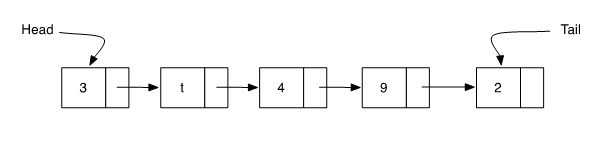
\includegraphics[width=0.5\textwidth]{pictures/linked_list.jpg}
\caption{Single Linked List}
\label{fig:single}
\end{figure}

   

\begin{figure}[H]
\centering
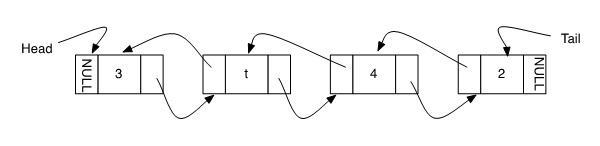
\includegraphics[width=0.5\textwidth]{pictures/double_linked_list.jpg}
\caption{Double Linked List}
\label{fig:double}
\end{figure}


\begin{figure}[H]
\centering
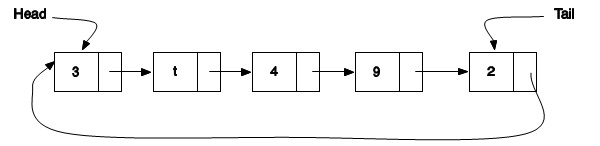
\includegraphics[width=0.5\textwidth]{pictures/circular_linked_list.jpg}
\caption{Circular Linked List}
\label{fig:circular}
\end{figure}

\subsection{Implementation Details}  

When you write the operations for a linked list, the most challenging aspect is to keep track of the pointers that give access to the adjacent nodes in the list.

The pseudocode below illustrates the process for adding an element to the beginning of the list. This pseudocode assumes that currentElement is the beginning of the list and that newElement has already been allocated and is pointing to the list data.  The order of these two lines of code is very important. Can you explain why?     

\begin{lstlisting}
       newElement-$>$next = currentElement-$>$next     
       currentElement-$>$next = newElement
\end{lstlisting}


The following steps are required to add a node to the end of the list:
\begin{enumerate}
\item Initialize a new element with the desired data.  This should be a separate function call.     
\item Walk through until end of list is reached 
\item Set the \textit{next} attribute of the element at the end of the list to the new element.    
\end{enumerate}

The most challenging part of this algorithm is  Step 2, walking through the list.   This is an operation that you will find yourself doing frequently with linked data structures.  The pseudocode for that step is shown below.  Draw a list on some paper and work through the algorithm until you understand how to walk through a list to get to the end of the list.

\begin{lstlisting}
currentElement = firstElementOfList //usually called the head of the list
while(currentElement->next is not NULL)
    currentElement = currentElement->next
lastElement = currentElement
\end{lstlisting}


\subsection{Nodes}
A node, or element,  is the fundamental  structure within a list. Regardless of your choice of implementation for a list, you will need some kind of a node structure to contain the data for the list.

When we take the time to create an ADT, we want it to be truly abstract.  That means that the ADT should not be tied to a particular kind of data, since the operations on a list are identical whether it is storing integers, strings, or structs.   It is a waste of time and testing to create separate ADT libraries for every possible type of data.

Instead we abstract the data by creating a data structure called a \textbf{node}.  As a minimum, the node contains  a pointer that points to the data being stored,  and a pointer to the next node in the list. 

\begin{lstlisting}
typedef struct Node {
    void * data;
    struct Node * next;
}Node;
\end{lstlisting}

The type of the data doesn't matter because it is cast to a void pointer (void *).   The data stored in the list might be a string; it might be an integer; or it might be a complex struct that represents a larger data record about some entity.

A linked list ADT should have a function that creates a new node,  sets the next pointer to NULL, and assigns the data to the data pointer.    Algorithms for working with linked lists assume that the \emph{\textit{next pointer}} for the tail element  is set to NULL so that the end of the list is easily identified.   It is very important to ensure that all new nodes have their next pointer initialized to NULL.

The data stored in a linked list is separate from the node definition.  A node simply points to the data element.  Suppose you were storing addresses in the list. The  data representation would then contain elements for name, phone number, mailing address and possibly email address.   A struct to represent the data might be given as follows.

\begin{lstlisting}
typedef struct Address {
    char * name;
    char * telephone;
    char * mailingAddress;
    char * email;
} Address;
\end{lstlisting}


\subsection{Operations}

A list ADT typically provides functions  that add elements to the list,  remove elements from the list,  report how long the list is,  and possibly sort the list.    It also must provide functions to create and destroy the list.

A minimum set of operations is shown below.  The names of the functions can vary, but an operation with comparable functionality is necessary.    The parameters given in the pseudcode are also a minimum set of parameters.  Implemented functions may need additional parameters. 

\begin{lstlisting}
·create(...): List
·destroy(List)
·insertFront(List,  DataElement):theHead
·getFront(List):DataElement
·deleteFront(List)
\end{lstlisting}


 Once a list is created, it is manipulated  through operations on the ADT functions. These functions and procedures  can do whatever the programmer desires, as long as they are written  carefully to \textbf{encapsulate} the implementation details of the list.   While a list ADT is functional with just the minimum set of functions, usually more functions are provided with an ADT.  Some common additional operations on lists include
 
 \begin{itemize} 
 \item Finding the length of a list
 \begin{itemize}
\item  returns an int and takes the root of the list as a parameter
  \item getLength(List):int
  \end{itemize}
\item Finding an element of a list
 \begin{itemize}
 \item returns a  pointer to the element in the list, without removing the element from the list
\item needs a search criteria and the list as parameters, and returns a pointer to the data element, not the node

\item find(Element, List)
\end{itemize}
\item  Printing a list.
\begin{itemize}
\item might print the entire list to stdout
\item a more elegant version returns a 
             string (or pointer to a string) that represents a nicely formatted 
             printout of the list elements.
\item print(List):char*
\end{itemize}
\item Adding/removing Nodes at the end of the  list

	\item  Adding/removing nodes after or before a 
         specific element
	\item Adding/removing nodes in a specific position in the list
	\item getting the length of the list
	\item {\textbf{Iterator} operations (current, next, previous, head, tail)
	
An iterator is a function that allows the user to step through the elements in a data structure.  Iterators typically “remember” the current position so that the user can move backwards and forwards within the data structure.

}
\end{itemize}

\subsection{Adding Elements}



 Elements can be added into a list at the 
       beginning, in the middle, at some arbitrary location, at the end, etc. 
       Each insert algorithm is slightly different than the others but the 
       basic idea is the same in all cases.


\begin{enumerate}
	\item Construct a new list element
	\item Put the desired data into the new element
	\item Find the location where the element is supposed to be inserted
	\item Adjust the other list elements so that the new one is in the right 
         location and so all existing elements are still part of the list
\end{enumerate}

 Algorithms for inserting an element in  the first position and last position are shown below.  The pseudocode or algorithm for inserting in a specific location is left as an exercise for you to do.


\begin{lstlisting}
insertFirst(List, Element):theHead
Also Known as:addFront, insertFront, addHead, etc
Purpose: To add an element to the list at the front of the list
Preconditions: An initialized list is available.  
PostConditions: The node containing the desired data is added to the front of the list, the length of the list is increased by one, the head of the list is set to point at the newly added element.

insertFirst(List, Element):theHead
     initialize a new node with the desired data
     set the next pointer of the new node to point at the first nod of the list
     set theHead  of the list to point at  the new node
\end{lstlisting}
   
\begin{lstlisting}
insertLast(List, DataElement):void
Also Known as: addBack, insertBack, addTail, etc
Purpose: To add an element to the list at the tail of the list
Preconditions: An initialized list is available.  The new node has the next pointer initialized to NULL
PostConditions: The node containing the desired data is added to the end of the list, the length of the list is increased by one.

insertLast(List, DataElement):void
	initialize a new element with the desired data.  
	walk through until end of list is reached 
	set the next attribute of the element at the end of the list to the new element.    
\end{lstlisting}

\subsection{Deleting Nodes}

Deleting nodes in a list  uses algorithms that are the reverse of adding nodes.  Nodes can be deleted from the front, the back, or any location in the list.   The simplest algorithms delete nodes from the front or the back of the list.  


\begin{lstlisting}
deleteFront(List):Element  //often a delete method returns the value it has deleted
Also Known As: deleteFirst, removeFront, removeFirst
Purpose: To remove the first element from the list and return it to the calling procedure
Preconditions: A non-empty list is available
PostConditions: The first element of the list is removed, the length of the list is decreased by one,  the removed element is returned.

deleteFirst(List):Element
    set a temporary pointer(temp) to point at the first node in the list
   set the head pointer of the list to point at the second node in the list
   set the next pointer of the temporary node (the former first node)  to be NULL
    return(temp->data)
\end{lstlisting}

\begin{lstlisting}
deleteFromBack(List):Element  //often a delete method returns the value it has deleted
Also Known As: deleteLast, removeBack,  etc
Purpose: To remove the last element from the list and return it to the calling procedure
Preconditions: A non-empty list is available
PostConditions: The last element of the list is removed, the length of the list is decreased by one,  the removed element is returned.

deleteLast(List):Element
	walk the list to find the second last element //node->next->next == NULL
    set a temporary pointer(temp) to point at the last node in the list
    set the next pointer of the second last element to NULL
   set the next pointer of the temporary node (the former last node)  to be NULL
    return(temp->data)
\end{lstlisting}


\subsection{Other Core List Operations}

\begin{lstlisting}
isEmpty(List):Boolean
Purpose: To determine if the list has any elements stored in it   
Preconditions: An initialized list is available
PostConditions: None

isEmpty(List):Boolean
    if theHead == NULL and theTail == NULL
    then return (true)
    else return (false)
\end{lstlisting}   


isFull() is a function that is only useful in situations where a list could be 
       full.  This might happen in situations where a specific amount of memory 
       has been allocated to the list.  In that case when the memory is full,  
       a reallocation must be effected before the list size can be increased by 
       adding another element.
\begin{lstlisting}
isFull():Boolean
Purpose:To determine if the list is filled to capacity
Preconditions: An initialized, non-empty list is available
PostConditions: None
   
isFull():Boolean
    if length == maxSize
    then return (true)
    else return (false)
\end{lstlisting}
       

\begin{lstlisting}
create(...): List
Purpose: Create a new List initialized to be empty
Inputs: the function pointers for functions to manage the data stored in the list
Preconditions: None
PostConditions: A new list is created and is empty

create(...):List
    create the struct to hold the list metadata (head, tail, function pointers, etc)
    assign NULL to head (and tail if necessary)
    assign function pointers
    return(List)
\end {lstlisting}


\begin{lstlisting}
destroy(List)
Purpose: To destroy a list, freeing memory if required
Preconditions: A list exists
PostConditions: The list is destroyed

destroy(List)
   for each node in the list
       delete the data in the node using function pointer
       delete the node
   delete the struct holding the list metadata
\end{lstlisting}
   




\section{Array implementation for a list}

The previous sections of this document have focussed on the list composed of linked data structures (the linked list).   A list ADT does not have to be a constructed using linked nodes.   An array can be used to construct a List ADT. At its simplest, the array holds the data in the list and each location in the array is one element of the list. The head of the list is at the first position in the array and the tail of the list is wherever the last element is.  

The array-based list stores void * data in the array in the same way that the linked node stored void * data for the linked data structure.

The choice of implementation does not change the operations required for the list ADT but it does change some of the implementation details.   For example,  if the user wished to insert data into the list maintaining a sorted order, the insert operation would require that room is made for the new element by shifting any subsequent elements one position in the array.   If a data value was to be deleted from the list,  the delete operation must ensure that the space left from the deletion is filled by shifting the tail-end of the array one space towards the head.     

Because arrays must be allocated to be a fixed size in C,  a new longer array must be constructed and the data copied into it if the list grows longer than the size of the array.

Fortunately,  because of information hiding and encapsulation,  the user of the the List ADT should never need to know whether the List is implemented as a linked data structure or an array-based list.


\section{ Array Lists vs Linked Lists}   

\textbf{Linked Lists}
\begin{itemize}
\item Advantages
\begin{itemize}
\item Linked lists can be an arbitrary size because the list grows and  shrinks as elements are added.     
\item Insertion and deletion of data do not require moving  other  data elements, so the operations are more efficient than the comparable operation  on an array structure. 
\end{itemize}
\item Disadvantages
\begin{itemize}
\item Linked lists are less efficient in situations where the program must be able to access any element of the data at any point in the program.  This type of accessibility is called \textbf{random access} and is more efficiently implemented with an array.
\end{itemize}    
\end{itemize}  

\textbf{Array Lists}
\begin{itemize}
\item Advantages
\begin{itemize}
\item Many operations are very fast because the array indices provide direct access
\item functions are simple and easy to debug, making ADT development simpler  
\end{itemize}
\item Disadvantages
\begin{itemize}
\item The resizing operations can be processor intensive if the list is large. There are many different strategies for deciding how much bigger to make the new array when resizing.    
\item To keep an array sorted, you must shuffle the elements each time you add another element.    
\end{itemize}
\end{itemize}

\section{List Iterator}

An iterator is a mechanism that allows navigation of a data structure.   An iterator is usually a different structure (or class in the case of object oriented programs)  that is fairly tightly coupled with the implementation of the data structure being iterated.

When creating an ADT library in C,  iterator functions can be included easily either with, or without the use of additional structures.

List iterator methods permit forwards and backwards navigation of the 
       list. They are extremely useful for accomplishing insertions and 
       deletions because the navigation code is encapsulated within the 
       iterator operation.

Iterator methods for a list might include:
\begin{itemize}
	\item next()
	\item previous()
	\item first()
	\item last()
	\item moveToNth()
	\item getCurrentElement()
	\item setCurrentElement()
\end{itemize}

While some of the iterator methods might seem to be duplicates of the basic list functions,  an iterator has an important role to play in encapsulation.     An iterator can hide the implementation of the list from the user of the library and can provide only the navigational functions to the user.

For example,  an iterator for a list could be set up as follows:

\begin{lstlisting}
typedef struct Iterator
{
    List * theList;
    Node * currentListPos;

}ListIterator;

\end{lstlisting}

Given this structure,  the functions shown above could take a ListIterator as a parameter and provide the user with data that is stored in the list.   Of course, the ListIterator would need to be initialized with enough parameters that it could, in turn, initialize the underlying list.

An algorithm for the \textit{next()} function is shown below.

\begin{lstlisting}
next(ListIterator):DataElement  
Purpose: To move to the next element in a list and return the value of that element
Preconditions: The List member of the ListIterator is non-empty
PostConditions: The currentListPos of the iterator is increased by one and the data stored at that node is returned

next(ListIterator):DataElement  
	if currentListPos is not the end of the list
	   dataToReturn = currentListPos->data
	   currentListPos = currentListPos->next
	return (dataToReturn)
\end{lstlisting}


Some list iterator operations, such as previous() are easier using a double linked list, but all operations are possible regardless of list implementation.   The algorithm for other list iterator operations are left as a practice exercise.

\section{Extending Activities}

\begin{itemize}

\item Write an algorithm for the addToLocation() operation.  This operation should add an element to the list at a specific location in the list (identified by a number). Use the same specification format as has been used to describe operations in this lesson. Include all necessary parameters and return values in the signature of your specification. Be sure to include preconditions and postconditions

\item Write the algorithm to delete a node from the nth position of a linked list.  The operation should return the deleted data and  ensure that the remaining elements of the list are properly connected.

\item Write the algorithm for inserting a node in sorted order given an array implementation of a list.   The algorithm should take the data as a parameter.

\item Write the algorithm for the list iterator operation \textit{previous()}.  It should take a ListIterator as a parameter and return the data associated with the previous node.  It should also adjust the current position pointer.   Write the algorithm for a double linked list and then write it again for a single linked list.

\end{itemize}

%%%%%%%%%%%%%%%%%%%%%%%%
%Stack chapter
%%%%%%%%%%%%%%%%%%%%%%%%

\chapter{Stack ADT}

    A full understanding of the List ADT is needed in order to fully understand stacks.  If you do not understand how lists work and the associated operations of lists, please review that material before attempting to understand the Stack ADT.
    
    
\begin{figure}[H]
\centering
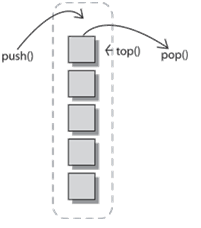
\includegraphics{pictures/stack.png}
\caption{A stack data structure}
\label{fig:stack}
\end{figure}


    A stack is a linear data structure  in which all insertions and
deletions occur at the head, or top of the stack. A stack ADT can only be
interacted with from the front, or top, of the stack. Items can be placed
on the top, and then taken off the top, but never shuffled or sorted
through. A stack of building blocks on a base is a good visual metaphor for
a stack. Imagine that you want to add height to the stack of blocks- you
 add blocks to the top of the stack. To reduce the height of the
stack of blocks, you  remove blocks from the stack.


\begin{figure}[H]
\centering
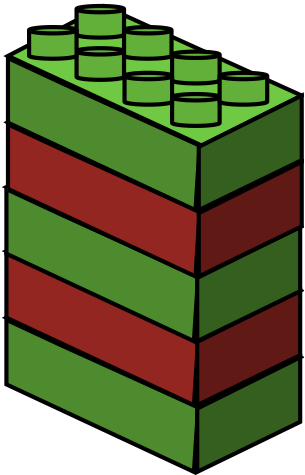
\includegraphics{pictures/stackofbricks.png}
\caption{A stack of bricks}
\label{fig:lego}
\end{figure}



Another good metaphor for a stack is a stack of pennies. If you want a penny of a specific year on top you could remove pennies from the stack until you reach it. If the penny you want is on the bottom of the stack you would need to remove every penny above it in order to get to it. You couldn’t just pull it out from beneath all the other pennies. And no, a stack implementation won’t let you knock over the stack and grab the penny you want.


\begin{figure}[H]
\centering
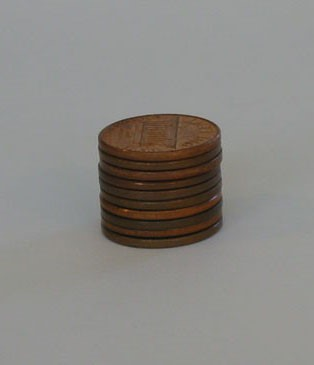
\includegraphics{pictures/pennies.jpg}
\caption{A stack of pennies}
\label{fig:pennies}
\end{figure}

\section{Why use stacks?}

Often programmers feel that if they have one usable data structure  that is enough.  The list ADT is powerful and flexible and many programmers use it for all purposes.  However, there are many times when a special purpose ADT is more appropriate.  Some applications do not require the flexibility of a list, but need to meet speed or data storage requirements.  A specialized ADT can often reduce overhead and speed up operations.  Below are some additional reasons to be familiar with and understand multiple different types of ADTs.

\begin{itemize}
\item A program becomes more readable and errors become easier to find therein if explicit use of specialized data structures is made. 
\item Simpler interfaces (like in the case of the class stack) make specialized implementations possible which are particularly time or space efficient. For example, the Stack ADT could be implemented with the help of a particularly space-efficient list ADT, thus reducing space requirements overall.  
\item The use of a specialized data structure often leads to more insight into the problem definition from which further improvements in the implementation can arise then. 
\item To give an example: That a given stack will store only a certain number of elements known in advance during the overall runtime could be noticed by the programmer only by explicit use of a stack. A b\_stack then would be the structure of choice and its use would imply an improvement of the space efficiency. 
\end{itemize}

\section{Operations on a Stack ADT}
    A Stack is a \textbf{LIFO data structure}. LIFO stands for Last In, First Out. The last element to be placed in the stack will be the first to be removed from it.   
    
    The most modular way to create a Stack ADT is to encapsulate a List ADT. 
To create a stack using an encapsulated list, you simply make use of the operations provided by the LIST ADT. For example, a list ADT might have operations such as addHead, removeHead. Those operations can be used inside the Stack ADT to provide the operations needed by the Stack. 
    Often a Stack ADT is implemented as a \textbf{wrapper}  around a List ADT.   In the same way that the ListIterator used the List ADT and provided  iterator operations to the user while hiding the details of the list from the user,  the Stack ADT uses the List ADT and provides stack operations.

A Stack ADT structure might look as follows:

\begin{lstlisting}
typedef struct Stack
{
    List * theList;
    Node * top;  //top of the stack
    int stackSize;
}Stack;

\end{lstlisting}

The operations provided with any Stack ADT must allow for creation and destruction of the stack as well as insertion and removal of elements as a minimum.   Because the goal is an \textbf{abstract} data type,  the stack must  be initialized with pointers to functions for managing the stored data.   

Since the Stack ADT presented here is a wrapper around a List ADT, most of the stack operations simply call the operations of the underlying list.  The Stack ADT hides the list operations from the user of the stack.

\begin{lstlisting}
create(): Stack
Purpose: To create and initialize a stack
PreConditions: None
PostConditions: A stack is created and initialized to empty

create(): Stack
      create the List sending in the appropriate function pointer parameters
     set the top  pointer to the first position in list
     return (the stack we just created)
\end{lstlisting}


\begin{lstlisting}
destroy(stack)
Purpose: To destroy a stack
PreConditions: An initialized stack exists
PostConditions: The stack is destroyed and all associated memory is freed.

destroy(Stack)
     destroy theList using the list ADT destroy function
     destroy the top pointer
     destroy the stack struct
\end{lstlisting}



The push() function of a stack is equivalent to the addFront() function for  a list.  One of  the  main purposes for creating the specialized ADT is program readability and maintainability so it is important to use function names that are widely associated with the specific ADT.

\begin{lstlisting}
push(Stack, Element)
Also Known As: add, insert
Purpose: Places an element in the stack
PreConditions: The stack is not full
PostConditions: An element is added to the stack, the length is increased by one, the top of the stack points to the newly added element

push(Stack, DataElement)
     insertFront(theList, DataElement)  
     top is set to the position of the data just added
     stackSize is increased by one
\end{lstlisting}


\begin{lstlisting}
pop(Stack): Element
Also Known As: remove, delete
Purpose: Removes the first element in the stack
PreConditions: The stack is not empty
PostConditions: The first (top) element of the stack is removed and returned to the caller. The top of the stack is set to the successor of the removed element, the length of the stack is decremented by one.

pop(Stack):Element
     theRemovedElement  is set to the return value of getFront(theList)
     the first element of the list is removed  by calling removeFront(theList)
     top  is set to  the new first element of theList 
     return(theRemovedElement)
\end{lstlisting}


\begin{lstlisting}
peek(Stack): Element
Also Known As: top
Purpose: To examine the element at the top of the stack without removing it from the stack.
PreConditions: The stack is not empty
PostConditions: Returns the element that is at the top of the stack but does not remove that element from the stack.

peek(Stack):Element
     theValue  is set to point at the data element at position (top) in the list. Sometimes a copy of the data element is made rather than providing a pointer to the actual data element.   Use the list operation getFront(List)
     return (theValue)
\end{lstlisting}




\begin{lstlisting}
isEmpty(Stack): Boolean
Purpose: To determine if the stack is empty
Preconditions: An initialized stack exists
PostConditions: evaluates to true if the stack has no elements, false otherwise

isEmpty(Stack):Boolean
     if(theList is empty)  //use the List isEmpty() function
     then return(true)
     else return(false)
\end{lstlisting}




\begin{lstlisting}
isFull(Stack): Boolean
Purpose: Relevant only in situations where the size of the stack is limited. Is used to determine whether the stack is full.
PreConditions: An initialized stack is available
PostConditions: Evaluates to true if the stack has reached its maximum size, false otherwise.

isFull(Stack):Boolean
     if(theList is full)  or the MAX_SIZE of the stack has been reached
     then return(true)
     else return(false)
\end{lstlisting}


The size of a stack is often an input that is used in algorithms involving a Stack ADT.  As such it is an important piece of data to keep, even if the underlying list implementation does not keep a length.   Stack operations may need to have logic added to update the stackSize struct member.

\begin{lstlisting}
length(Stack): int
Purpose: To obtain a count of the number of elements currently in the stack
PreConditions: An initialized stack is available
PostConditions: returns the count of the number of elements

length (Stack): Int
     return  stackSize  (or theList->length if the list ADT keeps track of length)
\end{lstlisting}



\section{Array Implementation of a Stack}
    Arrays can also be used to create a stack ADT. To use an array as a stack you simply need to ensure that the elements are added to the array sequentially and that your stack ADT keeps track of where the 'top' of the stack is in the array. 
    
 For example, suppose we allocated an array of size 8 to store a stack of
 integers, and a separate variable called top to keep track of the position of the top of the stack. The figure below shows the array after the integer 7 has been pushed onto the stack. The variable top has the value 0 because
    the top of the stack is at position 0 in the array.

\begin{figure}[H]
\centering
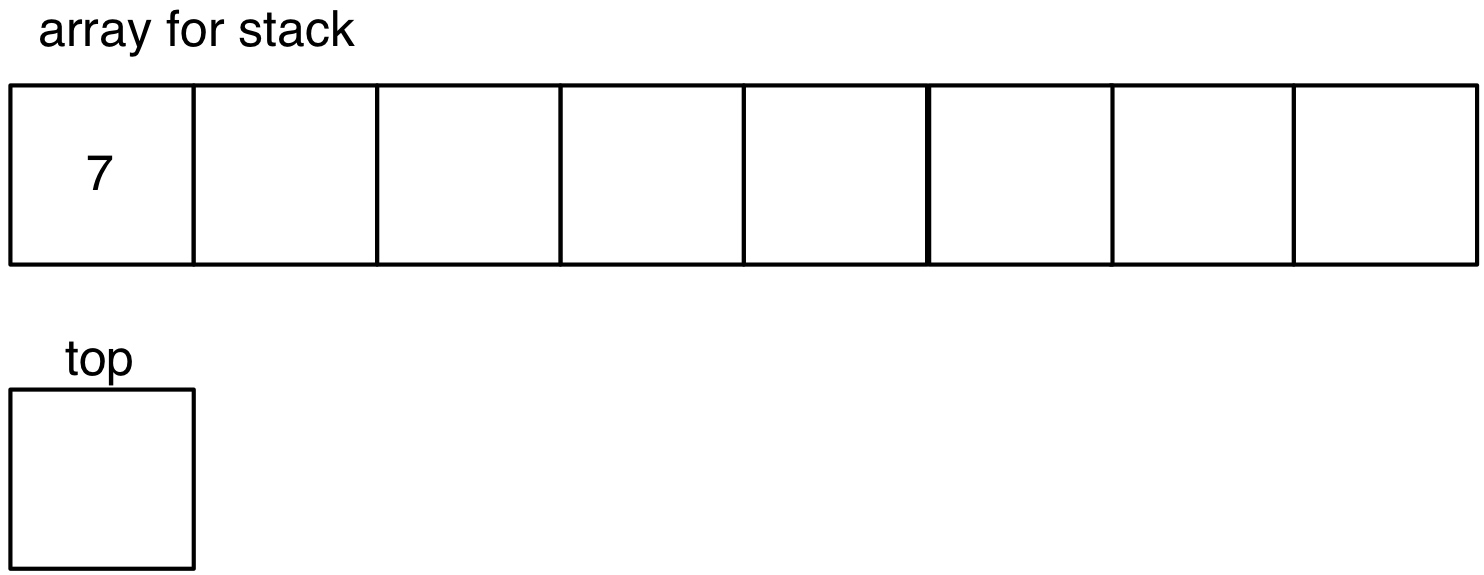
\includegraphics{pictures/arrayStackOne.jpg}
\caption{7 at position 0}
\label{fig:stack1}
\end{figure}
 After three more elements are pushed onto the stack, the array contains four items and the top variable holds the value of 3 because the top of the stack is at position 3 in the array.
\begin{figure}[H]
\centering
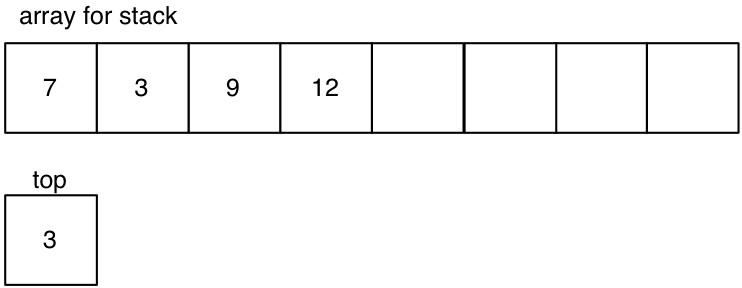
\includegraphics{pictures/arrayStacksTwo.jpg}
\caption{7 at position 3}
\label{fig:stack2}
\end{figure}


If an element is popped off the stack, the array then holds three elements and the top variable would hold the value 2 because the top of the stack moves to position 2 when an element is taken off the stack.

An array implementation of a Stack ADT needs to provide the same set of stack operations as the encapsulated list implementation.   However, the operations will not call list ADT operations, they will directly manipulate the array. Because an array is a fixed size, your ADT will need to provide an isFull operation so that programmers using your ADT can avoid overflowing your stack.

\section{Applications}
    A stack reverses the order of the elements stored. This property makes a
    stack very useful in certain programming applications including memory
    management and many mathematical applications

    It is always a good idea to use the correct data structure for the problem.
    While you could use a list for everything, the use of the more specialized
    data structures makes your code more readable and makes it much easier to
    see errors of logic. A specialized data structure can be created with
    efficiencies designed to make the program faster, or use less memory. Also,
    specialized data structures make it easier for the programmer using the ADT
    to conceptualize the problem. If a programmer is using a stack ADT for a
    program that requires the properties of a stack, then the programmer cannot
    make errors such as taking a data element out of the middle. 



\subsubsection{Reverse Polish Notation (Postfix notation)}
    The most common mathematical notation is \emph{infix} notation. The
    operators appear between the operands for the operation (e.g. 1 + 2, 5 *
    4, a/b). Infix notation is ambiguous by itself and must be annotated with
    parenthesis and a set of rules for the order in which operations are carried
    out.
    
    For example, consider the arithmetic problem 7 * 5 - 4 * 2. The answer
    could be 23 or 61 or ??. The 'right' answer is clear to those who
    understand the order of operations rules.

    A polish logician, Jan Lukasiewicz, developed a notation that does not
    require parenthesis and that embeds the required order of operations in the
    notation. Statements are read from left to right and the previous two
    operands are evaluated when an operator is encountered. The table below
    shows several examples of Infix and the equivalent Postfix notation. \newline

\begin{tabular}{lllll}
\hline
Infix           & Postfix   &  &  &  \\ \hline
a + b           & ab+       &  &  &  \\
(a-b)*c         & ab-c*     &  &  &  \\
(a+b)/(b*a)     & ab+ba*/   &  &  &  \\ \hline
(a*(b+c))/d     & abc+*d/   &  &  &  \\
a*((b-c)/(d+e)) & bc-de+/a* &  &  & 
\end{tabular}
    \newline Consider the second example. Reading left to right, the first two operands are a and b, the next character is a minus sign, so b is subtracted from a giving an answer that is stored as a single operand. The next item read is a c which is an operand. The next item read indicates multiplication so c is multiplied by the next most recent operand, which is the result of subtracting b from a.

    Work through each of the examples in the table so that you are confident in working with postfix notation.

    A stack is the data structure of choice for creating a reverse polish calculator. Each time you read a character from the input stream you push
it onto the stack. When an operation is encountered, you pop two operands
off the stack, perform the operation, and push the result back onto the stack. You then continue reading the input stream.

    Consider, once more, the second example in the table. As the input stream
is read, a is pushed onto the stack, followed by b. The next character is
an operand so two pop operations are executed and a-b is calculated. The
result is pushed onto the stack. At this point the stack contains one
value. The next symbol is read and is pushed onto the stack because it is
not an operand. There are now two elements on the stack. The final symbol
is read, two pop operations are executed and the multiplication operation
is executed.



\section{Resources}
    There are many good resources about stacks on the internet. A few are listed below, but this is only a small sample.   It is worth spending some time to find resources that work well for your personal style of learning.

\begin{itemize}
	\item http://www.cs.bu.edu/teaching/c/stack/array/
	\item http://www.algolist.net/Data\_structures/Stack
\end{itemize}


\section{Extending Activities}

\begin{itemize}
\item Would a double linked list or a single linked list be a better choice for encapsulation in a Stack ADT?  Justify your opinion.

\item Write the algorithms for push() and pop() given an array implementation of a stack.  Show the stack struct definition as  well.

\item Create a design or prototype of a reverse polish calculator program.   You should limit operations to + - * and /.    Use a stack ADT in your design.

\end{itemize}

%%%%%%%%%%%%%%%%%%%%%%%%%%%
%Queues
%%%%%%%%%%%%%%%%%%%%%%%%%%%


\chapter{Queues}
\section{Introduction}

A queue is an example of a \textbf{FIFO data structure}. FIFO stands for First In First Out.   The defining characteristic of a FIFO data structure is that 
the data that has been stored the longest is the next piece of data that will be returned by a 'get data' operation. FIFO data structures do not allow the user to retrieve specific pieces of data.


\begin{figure}[H]
\centering
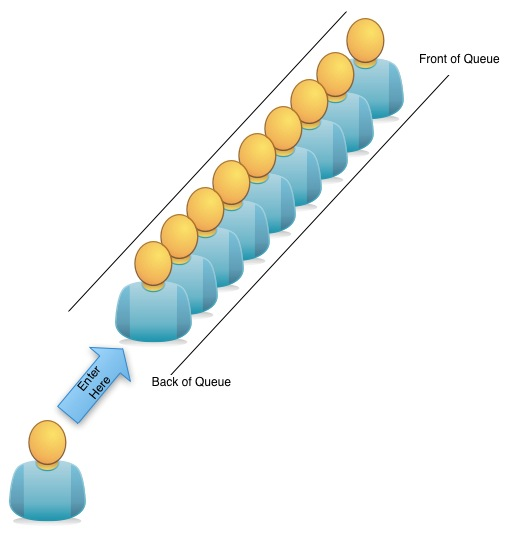
\includegraphics[width=0.5\textwidth]{pictures/queue.jpg}
\caption{Queue}
\label{fig:queue}
\end{figure}

A Queue ADT usually has no size restrictions and can grow or shrink unrestricted. In some applications it is possible to constrain the size of the queue to some predetermined maximum, which allows the software developer to select extremely efficient representations for the queue.

Similar to the Stack ADT, one of the most common implementations for a Queue is the encapsulation of a List ADT.   Because a Queue typically does not have a size, it is most common to use a linked list as the encapsulated ADT but an array implementation of a list could be used where max size is known and the characteristics of arrays give some needed performance advantage.

\section{Implementation: Encapsulate List ADT}

The most modular way to create a Queue ADT is to encapsulate a List ADT. To encapsulate an ADT you write your new ADT using the encapsulated one as a variable or data structure.

The Queue ADT must retrieve data elements from the front of the list (getFront(List)) and add elements at the back of the list (addToBack(List)).    If the chosen List ADT does not provide an addToBack function,  it cannot easily be used as the underlying ADT for a queue. 

 Encapsulation makes it possible to write the Queue ADT operations without worrying about the actual representation or memory management.  By using a good List ADT we ensure that the representation and memory management are handled properly, and we  make use of that to create our Queue.

%\begin{figure}[H]
%\centering
%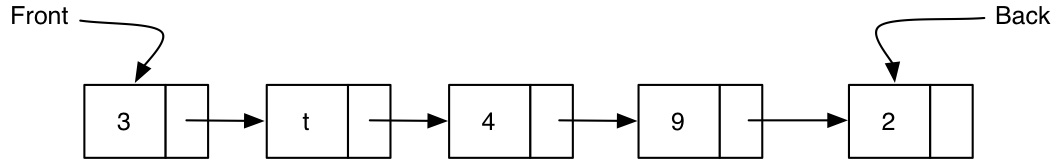
\includegraphics[width=0.5\textwidth]{pictures/linkedlistqueue.jpg}
%\caption{Linked List Queue}
%\label{fig:linkedListQueue}
%\end{figure}


The minimum set of operations on a Queue are:
\begin{itemize}
\item create()
\item enqueue()  //AKA add()
\item dequeue() //AKA remove()
\item destroy()
\end{itemize}


Other optional but useful operations allow the programmer to examine the front of the queue, determine the length of the queue, discover whether the queue is full or empty, etc.

The encapsulated Queue ADT is usually represented by a struct that is accompanied by several functions.  One possible representation of the struct is shown below.

\begin{lstlisting}
typedef struct Queue{
    List * theList;
    Node * front;
    Node * back;  //back is optional
    int * length;
}Queue;
\end{lstlisting}




\begin{lstlisting}
create(): Queue
Purpose: To create and initialize a queue
PreConditions: MAX\_LEN has been defined previously (it could be passed in as a parameter if desired)
PostConditions: A queue is created and initialized to empty


create(): Queue
     theList  is set to point at the return value from create a list- sending in the appropriate function pointers
     front  is set to point at the first position in list
     back  is set to point at the last position in list  //back is an optional pointer
     return (the queue  just created)
\end{lstlisting}




\begin{lstlisting}
destroy(Queue)
Purpose: To destroy a queue
PreConditions: An initialized queue exists
PostConditions: The queue is destroyed and all associated memory is 
       freed.

destroy(Queue)
     destroy theList using the list ADT destroy procedure
     destroy the front and back pointers
     destroy the Queue struct
\end{lstlisting}

   

\begin{lstlisting}
add(Queue, DataElement)
Also Known As: insert(), enqueue()
Purpose: adds an element to the end of the queue
PreConditions: The queue is not full
PostConditions: The new element is added as the last element in queue

add(Queue, Element)
      insertBack(theList, DataElement)
      back pointer is set last position of theList
      length of queue is updated
\end{lstlisting}


\begin{lstlisting}
remove(Queue):DataElement
Also Known As: delete(),  dequeue()
Purpose: removes the first element in the queue
PreConditions: The queue is not empty
PostConditions: The first (front) element of the queue is removed and 
       returned to the caller. The front of the queue is set to the successor 
       of the removed element.


remove (Queue): Element
     theRemovedElement <- getFront(theList)
     remove the first element from the list
     front is set to point at the new first element of theList
     length of the queue is updated
     return(theRemovedElement)
\end{lstlisting}





\begin{lstlisting}
peek(Queue):Element
Also Known As: front()
Purpose: To examine the element at the front of the queue without 
       removing it from the queue.
PreConditions: The queue is not empty
PostConditions: Returns the element that is at the front of the queue 
       but does not remove that element from the queue.

peek(Queue):Element
     return(getFront(theList)
\end{lstlisting}




\begin{lstlisting}
isFull(Queue):Boolean
Purpose: Relevant only in situations where the size of the queue is 
       limited. Is used to determine whether the queue is full.
PreConditions: An initialized queue is available
PostConditions: evaluates to true if the queue has reached its maximum 
       size, false otherwise.
       
isFull():Boolean
     if(theList is full)  OR MAX_SIZE has been reached
     then return(true)
     else return(false)
\end{lstlisting}

  


\begin{lstlisting}
isFull(Queue):Boolean
Purpose: To obtain a count of the number of elements currently in the 
       queue
PreConditions: An initialized queue is available
PostConditions: returns the count of the number of elements

isEmpty():Boolean
     if(theList is empty)
     then return(true)
     else return(false)
\end{lstlisting}




\begin{lstlisting}
length(Queue):int
Purpose: To obtain a count of the number of elements currently in the 
       queue
PreConditions: An initialized queue is available
PostConditions: returns the count of the number of elements

length(Queue):int
     return length OR length(List) if the list ADT provides a length function
\end{lstlisting}

\section{Array Implementation of a Queue}
Queues can be implemented using an array in much the same way as a Stack ADT can be implemented with arrays.

\begin{figure}[H]
\centering
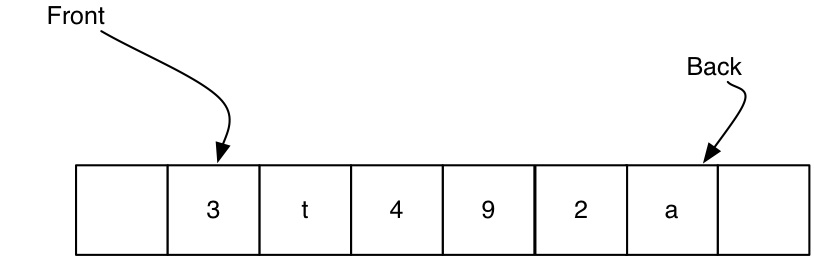
\includegraphics[width=0.5\textwidth]{pictures/arrayBasedQueue.jpg}
\caption{Array Queue}
\label{fig:arrayQueue}
\end{figure}

The programmer must keep track of the front and the back positions of the queue and, if a linear array is used, items must be shuffled up periodically in order to avoid using up all the memory in the computer.

In the example above, the array allocated to the queue has two empty spaces, one at the front and one at the back. One more element can be added to the back of the queue, and then all of the elements will need to be shuffled forwards in the queue in order to add a second additional element.

Removing the element 3 from this queue will free up one more space, but the entire set of elements will have to be shuffled forwards in order to use that space.


\begin{figure}[H]
\centering
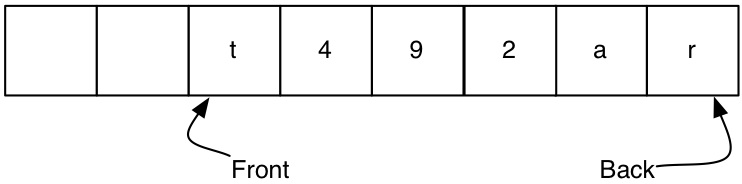
\includegraphics[width=0.5\textwidth]{pictures/arrayQueue2.jpg}
\caption{Array Queue Before Shuffling}
\label{fig:arrayQueue2}
\end{figure}

Shuffling the elements forward is a simple algorithm, but requires that every element is moved, which can take some time if the queue is several thousand elements long. The diagram below shows that there are two spaces at the end of the queue after elements are shuffled forwards.


\begin{figure}[H]
\centering
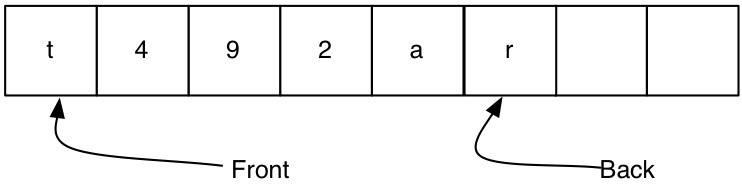
\includegraphics[width=0.5\textwidth]{pictures/arrayQueue3.jpg}
\caption{Array Queue After Shuffling}
\label{fig:arrayQueue3}
\end{figure}



While the array implementation is conceptually simple to describe to collaborators, it comes with several complications as well.  The array implementation can use extra memory if many items are added to the queue and then many are removed.  The queue must either be firmly limited in size or memory must be reallocated as the queue grows and memory reallocation affects the running time of the algorithm.

A common model for an array implementation of a queue is to use a circular buffer as the representation for the queue.

A circular buffer is really just an array, but the method of dealing  with the start and endpoints of the queue is slightly different. Imagine an array, but one that is arranged in a circle. Consider the picture below. The queue contains eight elements, beginning with an 'a'. After removing one element, and adding two more elements the queue will look like the second picture and has two spaces available for additional elements.

\begin{figure}[H]
\centering
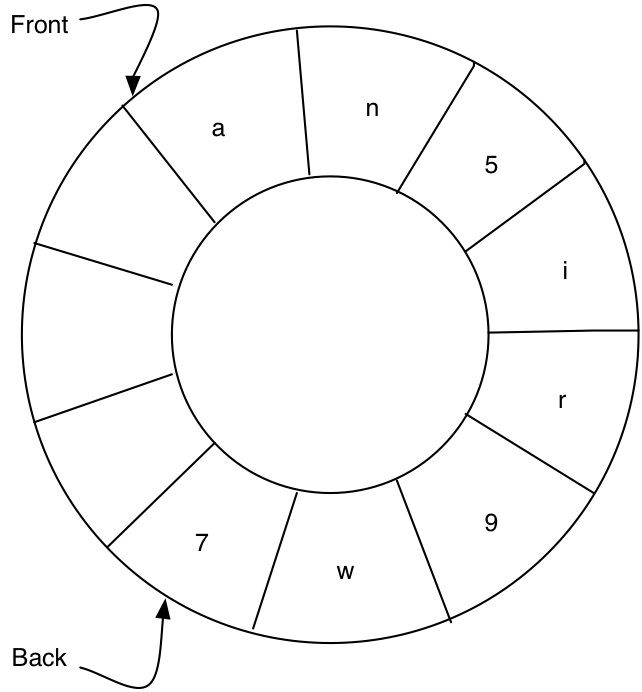
\includegraphics[width=0.3\textwidth]{pictures/circularbufferone.jpg}
\caption{Circular Buffer Queue Before}
\label{fig:circleQueue1}
\end{figure}

\begin{figure}[H]
\centering
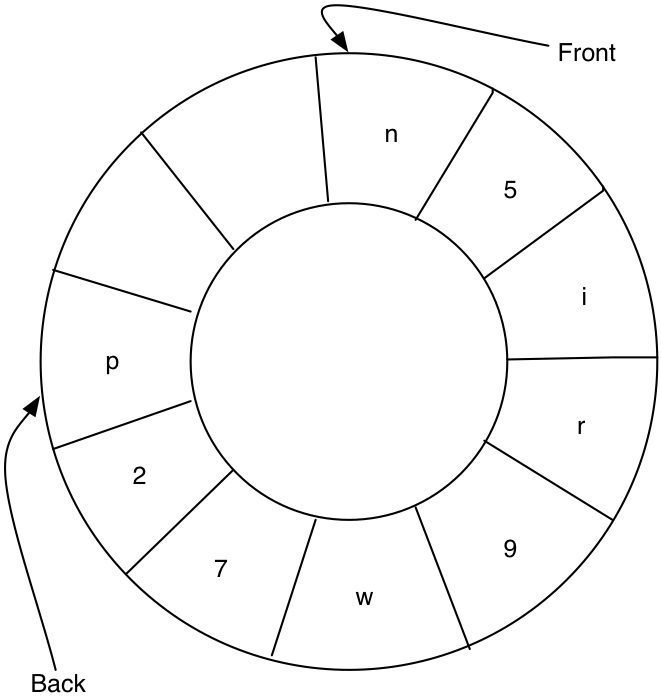
\includegraphics[width=0.3\textwidth]{pictures/circularbuffertwo.jpg}
\caption{Circular Buffer Queue After}
\label{fig:circleQueue2}
\end{figure}



One of the advantages of a circular buffer is that there is no need to shuffle elements around as there is with an array. One of the disadvantages is that the queue must be a fixed length, else the circular buffer suffers from the same memory reallocation requirements as a linear array implementation.

Of course, computer memory isn't circular, so a 'circular' buffer is really implemented using a linear array.


\section{Additional Resources}

\section{Extending Activities}

\begin{itemize}
\item Read the first few sections of the Computational Complexity chapter of this work.  Be sure you understand how to represent the complexity of an algorithm using \textbf{Big O} notation.     What is the complexity of the enqueue() and dequeue() operations?

\item What additional information must be kept track of in order to use a 
       conventional array as a circular buffer?  Give the Queue struct that you would use if you were writing a circular buffer queue implementation.

\item Write the algorithm for dequeuing an item from a circular buffer queue.

\item Which of the following statements about queues is untrue?

\begin{itemize}
\item a) Queues can have elements inserted at any position in the data 
       structure.

\item b) The first element inserted into a queue will be the first element 
       taken out of the queue.

\item c) Queues can be found in the real world.

\item d) The size of a queue data structure is bounded only by the size of the 
       computer memory.

\item e)A queue is somewhat similar to a stack.

\end{itemize}

\item Which List operation would be most likely to be the one encapsulated if you were writing a remove operation for a queue?
\begin{itemize}
\item a) addHead(elementToBeAdded)

\item b)length()

\item c)removeBack()

\item d)removeHead()

\item e)insert(position, elementToBeAdded)
\end{itemize}





\item Given the following queue:  A B b E r S T,  where A is the front of the 
       queue,  what will the queue content be after two remove operations?
\begin{itemize}
\item a)  A B b E r S T

\item b) b E r S T

\item c) A B b E r S

\item d)  T A B b E r S

\item e) The queue will be empty

\end{itemize}




Given the following queue: t y 5 8 i 2 d t e,  what should a call to 
       length() return?
\begin{itemize}
\item a)9

\item b) 8

\item c) 10

\item d) it will generate an error because of the mixed data types

\item e) 3
\end{itemize}

\end{itemize}
